% 2022 新高考Ⅱ卷 20：三棱锥 P-ABC（PO⊥底面 ABC，E 为 PB 的中点）
% 立体坐标 A(0,0,0)、B(4√3,0,0)、C(0,12,0)、O(2√3,2,0)、P(2√3,2,3)、E(3√3,1,3/2)。
% 画布投影：(x,y,z) -> x·(1,0) + y·(-0.22,0.46) + z·(0,1)，故 C 落在左上远处、O 在底面内部、P 在 O 正上方。
% 深度方向取得较陡，是为了让汇于远点 C 的五条连线张开成可辨的扇形。
% 虚线（被遮挡）：PO（竖直）、CB、CO、CE；其余为可见实线。
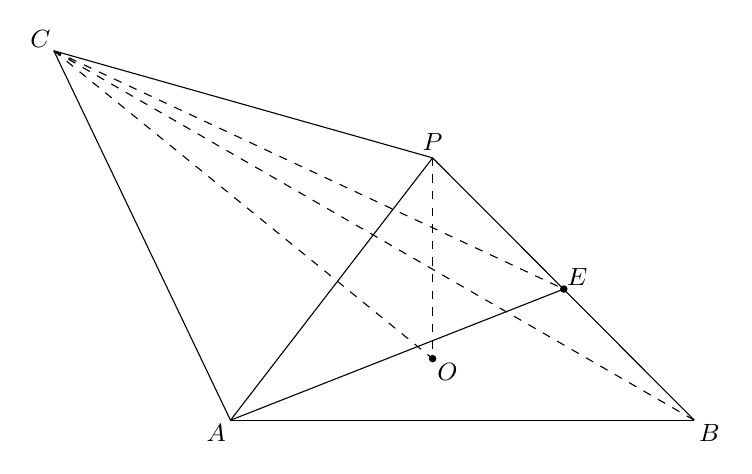
\begin{tikzpicture}[scale=0.85, font=\small]
  \coordinate (A) at (0,0);
  \coordinate (B) at (6.93,0);
  \coordinate (C) at (-2.64,5.52);
  \coordinate (O) at (3.02,0.92);
  \coordinate (P) at (3.02,3.92);
  \coordinate (E) at (4.98,1.96);
  % 可见实线
  \draw (A) -- (B);
  \draw (A) -- (C);
  \draw (P) -- (A)  (P) -- (B)  (P) -- (C);
  \draw (A) -- (E);
  % 被遮挡
  \draw[dashed] (P) -- (O);
  \draw[dashed] (C) -- (B)  (C) -- (O)  (C) -- (E);
  \fill (O) circle (1.6pt);
  \fill (E) circle (1.6pt);
  \node[below left,  inner sep=1.5pt] at (A) {$A$};
  \node[below right, inner sep=1.5pt] at (B) {$B$};
  \node[above left,  inner sep=1pt]   at (C) {$C$};
  \node[below right, inner sep=1.5pt] at (O) {$O$};
  \node[above,       inner sep=2.5pt] at (P) {$P$};
  \node[above right, inner sep=1pt]   at (E) {$E$};
\end{tikzpicture}
